\documentclass[12pt]{article}

\usepackage[13643]{easymcm}  % Team control number
\usepackage{longtable}
\usepackage{booktabs}

\problem{A}  % Problem number

\title{Paper Name}  % Title

\begin{document}

\begin{abstract}

	Some random text
	
\end{abstract}

\maketitle
\tableofcontents

\section{Introduction}

	\subsection{Problem Background}
		
		
		
	\subsection{Problem Restatement}
	
		some random text

\section{Dandelion Spread Model}

	\subsection{Assumptions and Justifications}
	
		\begin{enumerate}
			
			\item \textbf{The dandelion is located at the midpoint of an edge of a square field, which has dimensions of 100m$\times$100m (1 hectare).  When seeds are blown out of the field, they are neglected.}
			\vspace{-0.125in}
			\begin{description}
				\item[Justification:] The problem states that the dandelion is adjacent to the field.  Thus, we consider the dandelion to be located on the edge of the field.  Furthermore, we limit our consideration within the field.  Seeds that land outside the field are considered to be negligible, possibly due to a river or forest that borders the field.
			\end{description}
			
			\item \textbf{The field is an open field, with no plants that can hinder the spread of dandelions.}
			\vspace{-0.125in}
			\begin{description}
				\item[Justification:] This assumption means that: \textbf{a.} dandelion seeds are not intercepted by other plants; and \textbf{b.} dandelions do not have to compete with other plants.  To consider other plants, we would have to obtain data about the distribution, morphology, growth habits, etc., of the local plants, which would make our model too complex.
			\end{description}
			
			\item \textbf{Wind direction is uniformly distributed from 0$^\circ$ to 360$^\circ$.}
			\vspace{-0.125in}
			\begin{description}
				\item[Justification:] Though we could obtain data about wind direction, we decided not to use them.  Wind direction can be affected by many factors and is very variable.  Consequently, local wind directions may be different from those observed at a weather station.
				
				Moreover, we do not know on which edge the dandelion is located, and we cannot determine wind from which direction will blow the seeds into the field.  If wind direction is uniformly distributed, all directions are equivalent and we can let the dandelion be located on any of the edges.
			\end{description}
			
			\item \textbf{Dandelions do not die.}
			\vspace{-0.125in}
			\begin{description}
				\item[Justification:] Dandelions are resistant to drought and cold temperature.  When they are partly eaten, they can regrow from the taproot.  Therefore, it is relatively difficult for them to die.
				
				The death of dandelions can be caused by: \textbf{a.} insects or pathogens; \textbf{b.} humans (through herbicides or other methods); or \textbf{c.} extreme weather.  It is too difficult for us to obtain the data required for a., and it is very likely that, when dandelions are introduced as a non-native plant, it does not encounter natural enemies.  And for b. and c., we can consider a natural environment with no extreme weather conditions.  
			\end{description}
			
		\end{enumerate}
	
	\subsection{Environmental Factors}
	
		Variables table? : $\mu_T$, $\sigma_T$, $\mu_W$, $\sigma_W$, $\mu_H$, $k_T$, $k_H$, $k$, $T$, $t$, $v_h$
		
		Six locations in the US were chosen for analysis.  We consider five properties of the environment and obtained the data for the six chosen locations, as shown in [USE REFERENCE FOR TABLE].  
		
		Table: 6 locations and corresponding parameter values
		
		We calculate an adaption factor $k$ from $\mu_T$ and $\mu_H$.  First, we determine the adaption factors for temperature and humidity respectively, according to [USE REFERENCE FOR TABLE].
		
		Table: $\mu_T \to k_T$, $\mu_H \to k_H$
		
		Then, we calculate the mean value of $k_T$ and $k_H$, and normalize it so that $k \in [0, 1]$.
		
		\begin{equation}
			k = \frac12 \left( \frac{k_T + k_H}2 - 1 \right)
		\end{equation}
		
		We suppose that the temperature follows a sinusoidal curve, as shown in \ref{fig:temp}.  This helps us simplify 
		
		\begin{align}
			\mu_T &= \lim_{n \to \infty} \frac{1}{n} \sum_{k = 1}^{n} T(t_k) \notag \\
			&= \lim_{n \to \infty} \frac{1}{360} \sum_{k = 1}^{n} T(t_k) \Delta t \notag \\
			&= \frac1{360} \int_0^{360} (-A \cos{\frac{2\pi}{360} t} + B) \, \mathrm{d}t.
		\end{align}
		
		Similarly, we 
		
		\begin{equation}
			\sigma_T^2 = \frac1{360} \int_0^{360} \left[ (-A \cos{\frac{2\pi}{360} t} + B) - \mu_T \right] ^2 \mathrm{d}t.
		\end{equation}
		
		\begin{equation}
			T = -\sqrt2 \sigma_T \cos{\frac{2\pi}{360} t} + \mu_T
		\end{equation}
	
		\begin{figure}
			\centering
			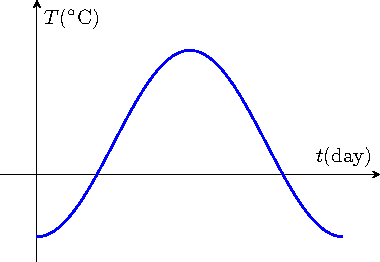
\includegraphics{fig-temperature_curve.pdf}
			\caption{Temperature curve}
			\label{fig:temp}
		\end{figure}
	
	\subsection{Dandelion Life Cycle}
	
		\begin{figure}
			\centering
			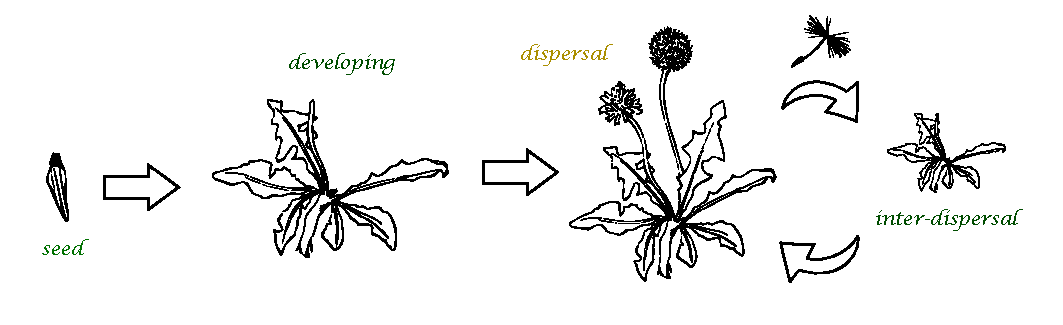
\includegraphics {life_cycle.pdf}
			\caption{Dandelion life cycle}
			\label{fig:lifeCycle}
		\end{figure}

	\subsection{Dispersal Distance}
		
		\begin{figure}
			\centering
			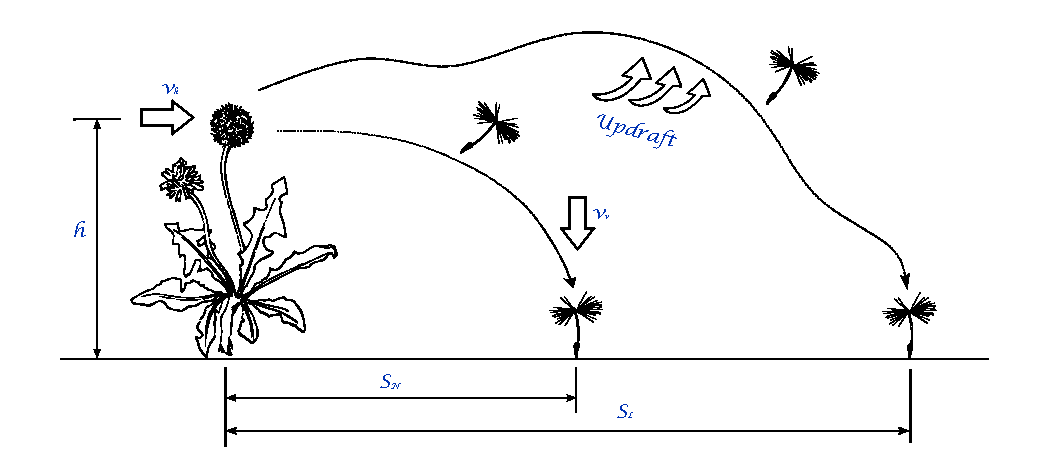
\includegraphics {wind_mode.pdf}
			\caption{Dandelion dispersal distance}
			\label{fig:dispersal}
		\end{figure}	
		
		\begin{equation}
			\frac{h}{v_v} = \frac{s_N}{v_h}
		\end{equation}
		
		\begin{equation}
			s_N = \frac{v_h}{v_v} h
		\end{equation}
		
		\begin{equation}
			\mathrm{P} (s_L < 0) = 1 - ae^{-0 \cdot b} = 0, \quad \mathrm{P} (s_L < 10) = 1 - ae^{- 10 b} = 1 - 0.5\%
		\end{equation}
		
		\begin{equation}
			\mathrm{P} (s_L < s) = 1 - e^{-0.53 s}
		\end{equation}
		
		We take $\max\{s_N, s_L\}$ to be the distance that the seed travels.
		
		\begin{figure}
			\centering
			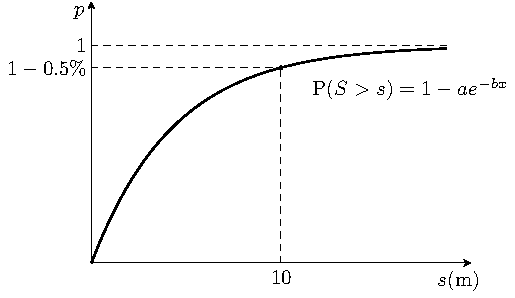
\includegraphics{fig-wind_curve.pdf}
			\caption{Cumulative distribution function of long-distance dispersal}
			\label{fig:longDistance}
		\end{figure}
		
	\subsection{Algorithm}
	
	\subsection{Dandelion Spread Results}
	
		\subsubsection{Results}
		
			text
			
			\begin{figure}
				\centering
				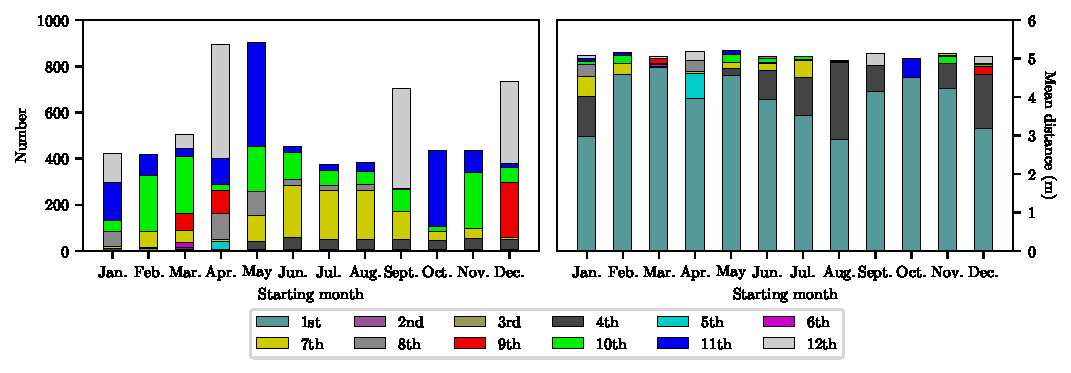
\includegraphics{start_month-number.pdf}
				\caption{Number and mean distance of dandelions in Florida when simulation starts at different times}
				\label{fig:start}
			\end{figure}
			
			\begin{figure}
				\centering
				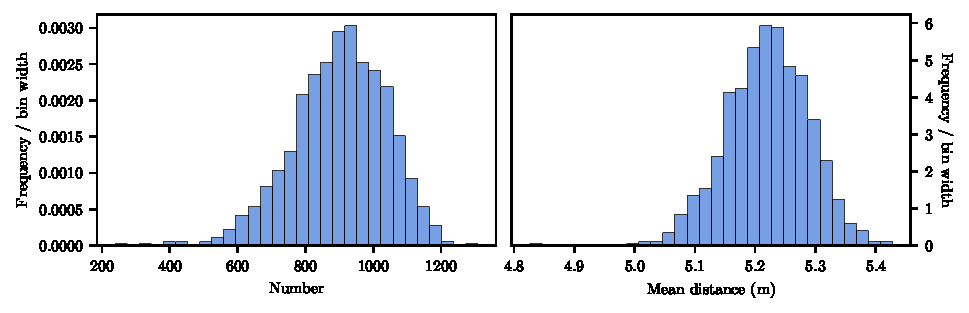
\includegraphics{number-frequency.pdf}
				\caption{Frequency distribution of number and mean distance of dandelions in Florida}
				\label{fig:freqDand}
			\end{figure}
			
			
			\begin{figure}
				\centering
				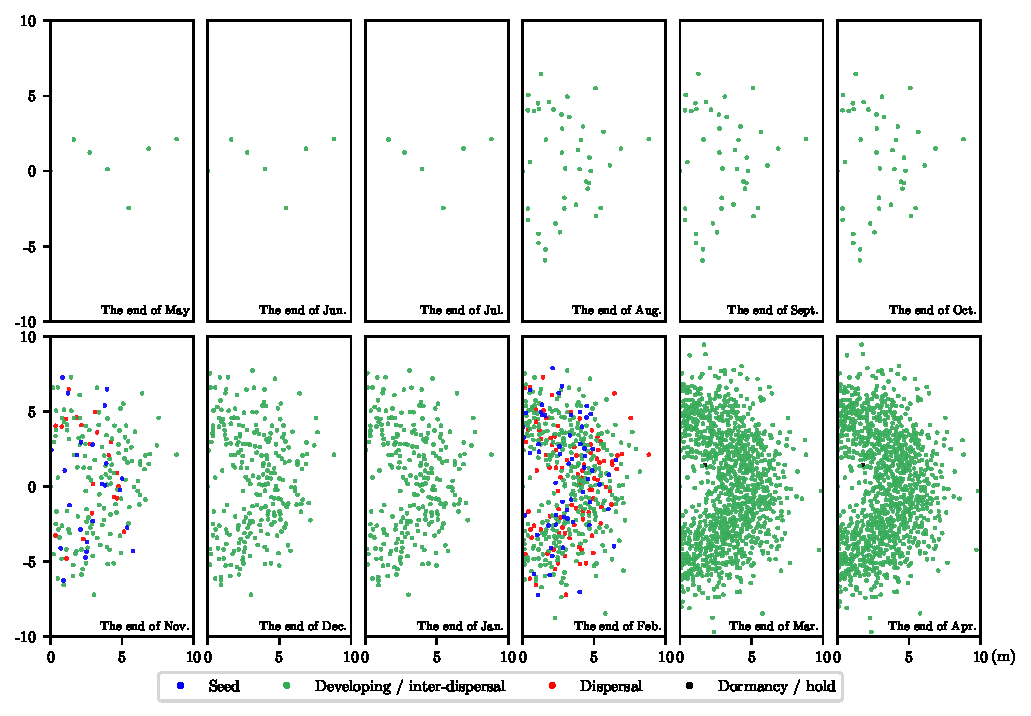
\includegraphics{spread_course-time.pdf}
				\caption{The spread of dandelion during a 12-month period in the District of Columbia}
				\label{fig:spreadDC}
			\end{figure}
			
			Lorem ipsum dolor sit amet Lorem ipsum dolor sit amet Lorem ipsum dolor sit amet Lorem ipsum dolor sit amet Lorem ipsum dolor sit amet Lorem ipsum dolor sit amet Lorem ipsum dolor sit amet Lorem ipsum dolor sit amet Lorem ipsum dolor sit amet Lorem ipsum dolor sit amet Lorem ipsum dolor sit amet Lorem ipsum dolor sit amet Lorem ipsum dolor sit amet Lorem ipsum dolor sit amet Lorem ipsum dolor sit amet Lorem ipsum dolor sit amet Lorem ipsum dolor sit amet Lorem ipsum dolor sit amet Lorem ipsum dolor sit amet Lorem ipsum dolor sit amet Lorem ipsum dolor sit amet Lorem ipsum dolor sit amet Lorem ipsum dolor sit amet Lorem ipsum dolor sit amet Lorem ipsum dolor sit amet Lorem ipsum dolor sit amet Lorem ipsum dolor sit amet Lorem ipsum dolor sit amet Lorem ipsum dolor sit amet Lorem ipsum dolor sit amet Lorem ipsum dolor sit amet Lorem ipsum dolor sit amet Lorem ipsum dolor sit amet Lorem ipsum dolor sit amet Lorem ipsum dolor sit amet Lorem ipsum dolor sit amet Lorem ipsum dolor sit amet Lorem ipsum dolor sit amet Lorem ipsum dolor sit amet Lorem ipsum dolor sit amet Lorem ipsum dolor sit amet Lorem ipsum dolor sit amet Lorem ipsum dolor sit amet Lorem ipsum dolor sit amet Lorem ipsum dolor sit amet Lorem ipsum dolor sit amet Lorem ipsum dolor sit amet Lorem ipsum dolor sit amet Lorem ipsum dolor sit amet Lorem ipsum dolor sit amet Lorem ipsum dolor sit amet Lorem ipsum dolor sit amet Lorem ipsum dolor sit amet Lorem ipsum dolor sit amet Lorem ipsum dolor sit amet Lorem ipsum dolor sit amet Lorem ipsum dolor sit amet Lorem ipsum dolor sit amet Lorem ipsum dolor sit amet Lorem ipsum dolor sit amet 
			
			\begin{figure}
				\centering
				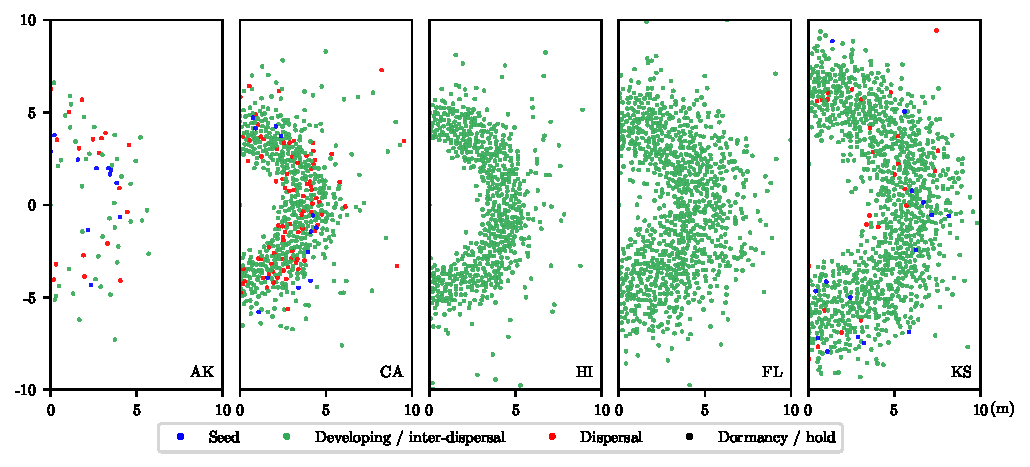
\includegraphics{spread_course-location_non_DC.pdf}
				\caption{The spread of dandelions at the end of 12 months at different locations}
				\label{fig:scatter5loc}
			\end{figure}
			
			Lorem ipsum dolor sit amet Lorem ipsum dolor sit amet Lorem ipsum dolor sit amet Lorem ipsum dolor sit amet Lorem ipsum dolor sit amet Lorem ipsum dolor sit amet Lorem ipsum dolor sit amet Lorem ipsum dolor sit amet Lorem ipsum dolor sit amet Lorem ipsum dolor sit amet Lorem ipsum dolor sit amet Lorem ipsum dolor sit amet Lorem ipsum dolor sit amet Lorem ipsum dolor sit amet Lorem ipsum dolor sit amet
			
					
			\begin{figure}
				\centering
				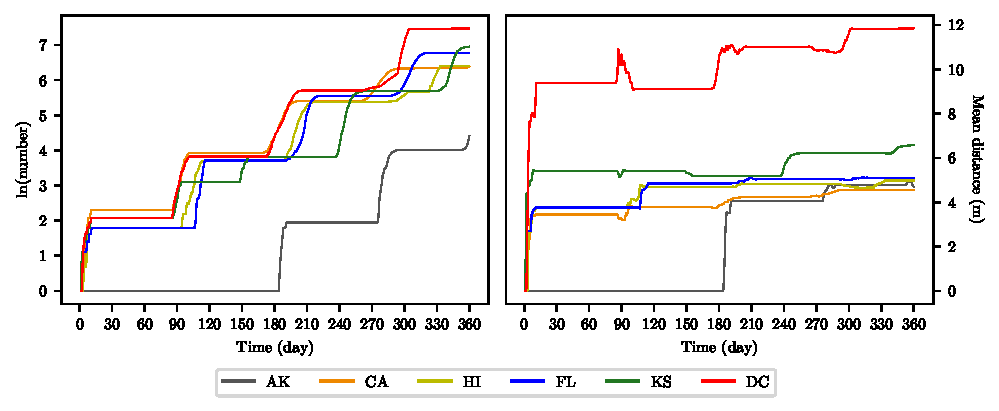
\includegraphics{number_mean_distance-time.pdf}
				\caption{Number and mean distance of dandelions plotted against time}
				\label{fig:time}
			\end{figure}
		
		\subsubsection{Sensitivity Analysis}
		
			\begin{figure}
				\centering
				\begin{minipage}{0.04\textwidth}\end{minipage}
				\begin{minipage}{0.46\textwidth}
					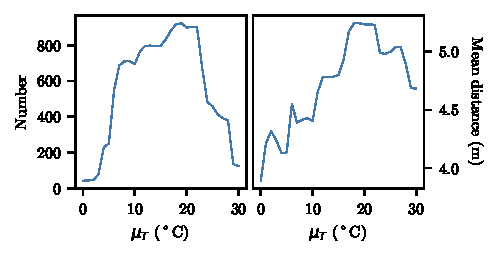
\includegraphics{sa_MuT.pdf}
				\end{minipage}
				\begin{minipage}{0.46\textwidth}
					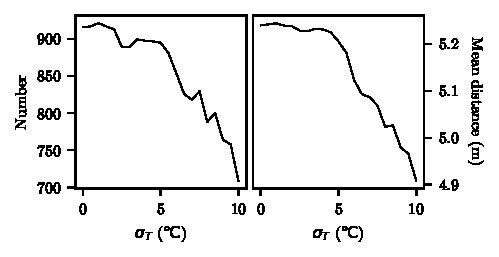
\includegraphics{sa_StdT.pdf}
				\end{minipage}
				\begin{minipage}{0.04\textwidth}\end{minipage}
				
				\begin{minipage}{0.04\textwidth}\end{minipage}
				\begin{minipage}{0.46\textwidth}
					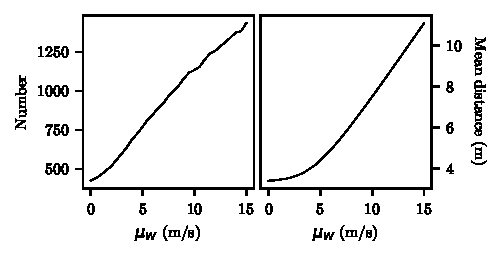
\includegraphics{sa_MuW.pdf}
				\end{minipage}
				\begin{minipage}{0.46\textwidth}
					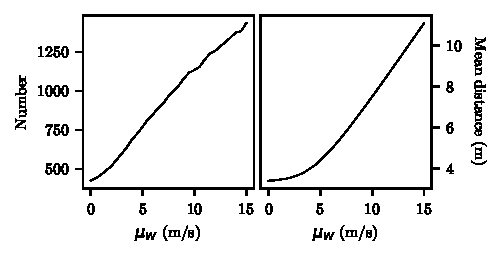
\includegraphics{sa_MuW.pdf}
				\end{minipage}
				\begin{minipage}{0.04\textwidth}\end{minipage}
				
				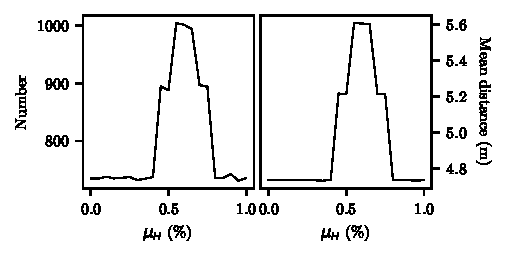
\includegraphics{sa_Hum.pdf}
				\caption{Sensitivity analysis}
				\label{fig:sa}
			\end{figure}
			
		\subsubsection{Strengths and Weaknesses}
		
	\subsection{Dandelion Spread Fitting Model}
		
		\subsubsection{Data}
		
		\subsubsection{Algorithm}
		
		\subsubsection{Results}
		
		\subsubsection{Sensitivity Analysis}
		
		\subsubsection{Strengths and Weaknesses}
	
			some random text
		
\section{Plant Impact Factor Model}

	\subsection{Assumptions and Justifications}
	
	\subsection{Model Description}

		hello
		
		{
			\fontsize{10}{14}\selectfont
			{
			\begin{longtable}{p{0.2in}p{1.5in}p{4.3in}}
			
				\toprule
				\multicolumn{1}{c}{\textbf{Symbol}} 
					& \multicolumn{1}{c}{\textbf{Aspect}}
					& \multicolumn{1}{c}{\textbf{$a_i$, $b_i$ and $c_i$ Evaluation}} \\
			
				\toprule
				\multicolumn{3}{l}{Category $A$ - Plant Characteristics}\\
				\midrule
				
				$A_1$ & Duration & $a_1=0.5$ (Annual), $0.75$ (Biennial), $1$ (Perennial)\\
				$A_2$ & Growing Habit & $a_2=0$ (Tree), $0.25$ (Shrub), $0.5$ (Vine), $0.75$ (Graminoid), $1$ (Forb/herb)\\ 
				$A_3$ & Growth Rate & The growth rate after successful establishment\\
					&& $a_3=0.5$ (Slow), $0.75$ (Moderate), $1$ (Rapid)\\
				$A_4$ & Lifespan & $a_4=0.25$ (when $a_1=0.5$ or $0.75$), $0.5$ (Short), $0.75$ (Moderate), $1$ (Long) \\
				$A_5$ & Fertility Requirement & Relative level of nutrition (N, P, K) required for normal growth and development.\\
					 && $a_5=0.5$ (Low), $0.75$ (Medium), $1$ (High)\\
				$A_6$ & Fruit/Seed Abundance & The amount of seed produced.\\
					&& $a_6=0.25$ (None), $0.5$ (Low), $0.75$ (Medium), $1$ (High)\\
				$A_7$ & Propagated Methods & The propagetion methods number, $n_7$. The methods can be Propagated by Bare Root, by Bulb, by Container, by Corm, by Cuttings, by Seed, by Sod, by Sprigs, or by Tubers. \\
					&& $a_7=0.25$ ($n_7=1$), $0.5$ ($n_7=2$), $0.75$ ($n_7=3$), $1$ ($n_7\geq4$)\\
				$A_8$ & Seed Spread Rate & The capability of the plant to spread through its seed production.\\
					&& $a_8=0.25$ (None), $0.5$ (Slow), $0.75$ (Moderate), $1$ (Rapid)\\
				$A_9$ & Seedling Vigor & The expected seedling survival percentage of the plant\\
					&& $a_9=0.5$ (Low), $0.75$ (Medium), $1$ (High)\\
				
				\midrule
				\multicolumn{3}{l}{Category $B$ - Human and Environment}  \\
				\midrule
				
				$B_1$ & Toxicity & The relative toxicity of the plant to either humans or livestock.\\
					&& $b_1=0$ (None), $0.5$ (Slight), $0.75$ (Moderate), $1$ (Severe)\\
				$B_2$ & Product & The level of the plant known to be suitable for multiple types of products.\\
					&& $b_2=0$ (Copiousness), $0.25$ (Many), $0.5$ (Some), $0.75$ (few), $1$ (None)\\
				$B_3$ & Palatable Animal & The relative palatability of this plant to browsing animals or to grazing animals.\\
					&& $b_3=0$ (High), $0.5$ (Moderate), $0.75$ (Low), $1$ (None)\\
				$B_4$ & Palatable Human & The plant produce berries, nuts, seeds, or fruits are palatable to humans. \\
					&& $b_4=0.5$ (Yes), $1$ (No)\\
				$B_5$ & Commercial Availability & The plant propagules are in the commercial marketplace \\
					&& $b_5=0.5$ (Yes), $1$ (No)\\
			
				\midrule
				\multicolumn{3}{l}{Category $C$ - Location}  \\
				\midrule
				
				$C_1$ & Soil Adaption & The soil is suitable for the plane\\
					&& $c_1=0.5$ (Yes), $1$ (No)\\
				$C_2$ & Temperature Adaption & The temperature is suitable for the plane\\
					&& $c_2=0.5$ (Yes), $1$ (No)\\
				$C_3$ & Humid Adaption & The humid is suitable for the plane\\
					&& $c_3=0.5$ (Yes), $1$ (No)\\
				$C_4$ & Population Density & The level of population density.\\
					&& $c_4=0.5$ (High), $1$ (Medium), $1$ (Low)\\
			
				\bottomrule
			
			\end{longtable}
			}
		}
		
		{
			\fontsize{10}{18}\selectfont
			{
				\begin{longtable}{c|ccccccccc|ccccc||cccc}
					\toprule
					&$A_1$&$A_2$&$A_3$&$A_4$&$A_5$&$A_6$&$A_7$&$A_8$&$A_9$&$B_1$&$B_2$&$B_3$&$B_4$&$B_5$&$C_1$&$C_2$&$C_3$&$C_4$\\
					\toprule
					$A_1$&$1$&$1/3$&$1/7$&$1/3$&$1$&$1/7$&$1/4$&$1/7$&$1/5$&$1/9$&$1/5$&$1/3$&$1/4$&$1/4$&$1/5$&$1/5$&$1/5$&$1/3$\\
					$A_2$&$3$&$1$&$1/5$&$1$&$3$&$1/5$&$1/2$&$1/5$&$1/3$&$1/7$&$1/3$&$1$&$1/2$&$1/2$&$1/3$&$1/3$&$1/3$&$1$\\
					$A_3$&$7$&$5$&$1$&$5$&$7$&$1$&$4$&$1$&$3$&$1/3$&$3$&$5$&$4$&$4$&$3$&$3$&$3$&$5$\\
					$A_4$&$3$&$1$&$1/5$&$1$&$3$&$1/5$&$1/2$&$1/5$&$1/3$&$1/7$&$1/3$&$1$&$1/2$&$1/2$&$1/3$&$1/3$&$1/3$&$1$\\
					$A_5$&$1$&$1/3$&$1/7$&$1/3$&$1$&$1/7$&$1/4$&$1/7$&$1/5$&$1/9$&$1/5$&$1/3$&$1/4$&$1/4$&$1/5$&$1/5$&$1/5$&$1/3$\\
					$A_6$&$7$&$5$&$1$&$5$&$7$&$1$&$4$&$1$&$3$&$1/3$&$3$&$5$&$4$&$4$&$3$&$3$&$3$&$5$\\
					$A_7$&$4$&$2$&$1/4$&$2$&$4$&$1/4$&$1$&$1/4$&$1/2$&$1/4$&$1/2$&$2$&$1$&$1$&$1/2$&$1/2$&$1/2$&$2$\\
					$A_8$&$7$&$5$&$1$&$5$&$7$&$1$&$4$&$1$&$3$&$1/3$&$3$&$5$&$4$&$4$&$3$&$3$&$3$&$5$\\
					$A_9$&$5$&$3$&$1/3$&$3$&$5$&$1/3$&$2$&$1/3$&$1$&$1/5$&$1$&$3$&$2$&$2$&$1$&$1$&$1$&$3$\\
					\midrule
					$B_1$&$9$&$7$&$3$&$7$&$7$&$3$&$4$&$3$&$5$&$1$&$5$&$7$&$4$&$4$&$5$&$5$&$5$&$7$\\
					$B_2$&$5$&$3$&$1/3$&$3$&$5$&$1/3$&$2$&$1/3$&$1$&$1/5$&$1$&$3$&$2$&$2$&$1$&$1$&$1$&$3$\\
					$B_3$&$3$&$1$&$1/5$&$1$&$3$&$1/5$&$1/2$&$1/5$&$1/3$&$1/7$&$1/3$&$1$&$1/2$&$1/2$&$1/3$&$1/3$&$1/3$&$1$\\
					$B_4$&$4$&$2$&$1/4$&$2$&$4$&$1/4$&$1$&$1/4$&$1/2$&$1/4$&$1/2$&$2$&$1$&$1$&$1/2$&$1/2$&$1/2$&$2$\\
					$B_5$&$4$&$2$&$1/4$&$2$&$4$&$1/4$&$1$&$1/4$&$1/2$&$1/4$&$1/2$&$2$&$1$&$1$&$1/2$&$1/2$&$1/2$&$2$\\
					\midrule
					\midrule
					$C_1$&$5$&$3$&$1/3$&$3$&$5$&$1/3$&$2$&$1/3$&$1$&$1/5$&$1$&$3$&$2$&$2$&$1$&$1$&$1$&$3$\\
					$C_2$&$5$&$3$&$1/3$&$3$&$5$&$1/3$&$2$&$1/3$&$1$&$1/5$&$1$&$3$&$2$&$2$&$1$&$1$&$1$&$3$\\
					$C_3$&$5$&$3$&$1/3$&$3$&$5$&$1/3$&$2$&$1/3$&$1$&$1/5$&$1$&$3$&$2$&$2$&$1$&$1$&$1$&$3$\\
					$C_4$&$3$&$1$&$1/5$&$1$&$3$&$1/5$&$1/2$&$1/5$&$1/3$&$1/7$&$1/3$&$1$&$1/2$&$1/2$&$1/3$&$1/3$&$1/3$&$1$\\
					\bottomrule
				\end{longtable}
			}
		}	

		hello!!! \\

		{
			\fontsize{10}{14}\selectfont
			{
				\begin{longtable}{cccccccc}
					\toprule
					Impact Factor&Attribute Number&max eigenvalue 
					&\multirow{2}{*}{$\mathrm{CI}=\frac{\lambda_{max}-n}{n-1}$}
					&\multirow{2}{*}{$\mathrm{RI}$}
					&\multirow{2}{*}{$\mathrm{CR}=\frac{\mathrm{CI}}{\mathrm{RI}}$}
					&\multirow{2}{*}{$\mathrm{CR}<0.1?$}\\
					Type&$n$&$\lambda_{max}$\\
					\toprule
					Global&$14$&$14.501$&$0.0386$&$1.49$&0.0259&Yes\\
					Local&$18$&$18.561$&$0.0330$&$1.49$&0.0221&Yes\\
					\bottomrule
				\end{longtable}
			}
		}	

	hello!!! \\

	\subsection{Sensitivity Analysis}
	
		\begin{figure}
			\centering
			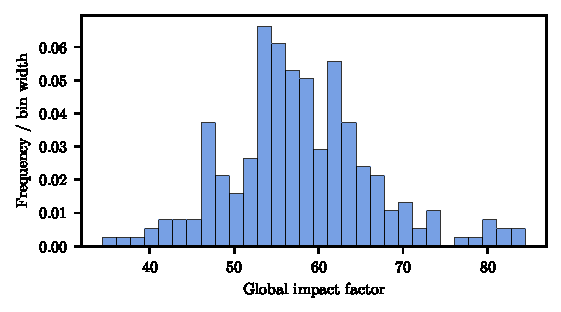
\includegraphics{IF-frequency.pdf}
			\caption{Frequency distribution of global impact factor}
			\label{fig:freqIF}
		\end{figure}
	
		\begin{figure}
			\centering
			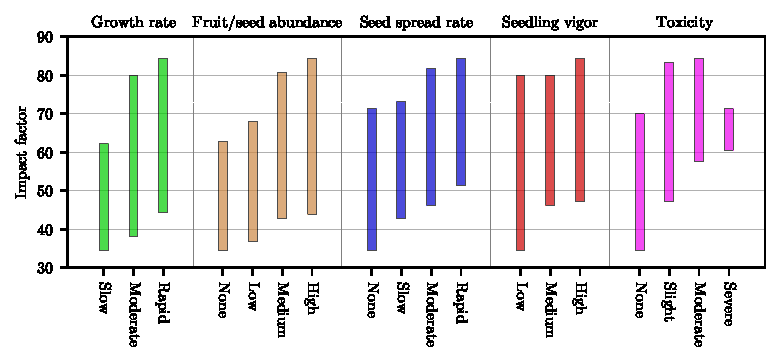
\includegraphics{categories-IF.pdf}
			\caption{What caption should this figure have?}
			\label{fig:IFfactors}
		\end{figure}
		
		\begin{figure}
			\centering
			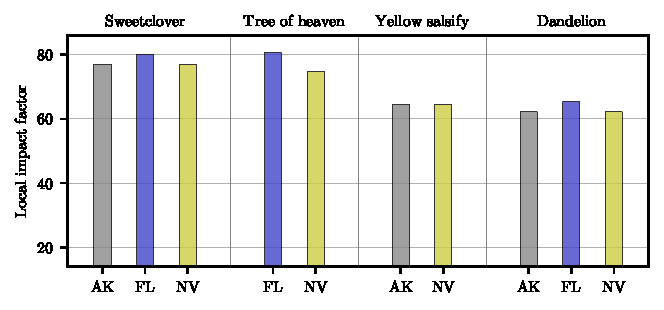
\includegraphics{IF_local-loc.pdf}
			\caption{What caption should this figure have?}
			\label{fig:IFLocal}
		\end{figure}
		
	\subsection{Strengths and Weaknesses}

		some random text
	
\section*{We Share the Earth}
\addcontentsline{toc}{section}{We Share the Earth}



\newrefcontext
\printbibliography

\end{document}
